\documentclass[12pt, a4paper]{article}
\title{\textbf{Laser Pointer Based Human-Computer-Interaction using Computer-Vision}}

\usepackage[labelformat=empty]{caption}
\usepackage{graphicx}
\usepackage{indentfirst}
\usepackage{wrapfig}
\usepackage{listings}
\usepackage{hyperref}
\usepackage{mathtools}
\usepackage{pgfgantt}
\usepackage{tocloft}
\usepackage{tocbibind}

\hypersetup{
	hidelinks = true
}
		

\begin{document}
	\listoffigures
	\pagenumbering{roman}
	\newpage
	\tableofcontents 
	\newpage
	\pagenumbering{arabic}

\section{Introduction}
\subsection{Background}
According to the \textbf{ICT (Information and Communication Technology) Master Plan 2013-2017}, the long term goal of education in Nepal is to provide citizens with appropriate knowledge, skills and attitude to work actively in the development of the country and to integrate Nepal into the global community through ensuring equitable access to and quality of education for all. In this context, the Ministry of Education has considered the use of Information and Communication Technology is essential to achieve the goals of education. And the prime components of it are:
\begin{itemize}

\item ICT infrastructure including internet connectivity
\item Human resources well trained in the use of the ICT infrastructure
\item Availability of the Teaching Learning Materials in the ICT infrastructure
\item System Enhancement procedures

\end{itemize}

Additionally, \textbf{Village Tech Solutions (VTS)} which was established in the year 1996 by \textbf{David} and \textbf{Hyadi Sowerwine}, with the mission to provide safe, efficient and inexpensive energy systems for the people of rural Nepal. VTS had been endeavoring to bring audio-visual system to the classrooms of Nepal to enhance their current education since the year 2008. By introducing such multimedia systems into the classroom, their aim is to make standard learning materials available to all Nepalese students irrespective of their socio-economic statuses. The information that can be gained from the introduction of such multi-media to rural villages can help not only the standard of education, but also the standard of living. This device has been named \textbf{Looma}, and it runs a Looma software comprising of a UI with all the teaching materials.  

Looma is a portable projection system that uses a wand to navigate the screen, like an interactive projector. Looma is an affordable and low power consuming audio-visual technology device which will provide an interactive window to internet and access to educational contents to village schools that have never seen computers, or in some cases, even books. And now with the release of ICT master plan for education, the government of Nepal has been cooperating with VTS regarding the same. Also, VTS has been collaborating with students and enthusiasts for the optimization of Looma, with the main aim to make Looma affordable, less power consuming and efficient, so that the people of rural communities can derive maximum advantage from it.  


\newpage

\section{Objectives:}

The basic objectives of our project is the modification of Project Looma in aspects listed below:

\begin{itemize}
	\item To make prototype for an alternative type of vision-based HCIs (Human Computer Interaction)
	\item To use laser pointer instead of IR (Infra-red) based interactive tool
	\item To remove the Wii technology, and its dependencies used in current prototype thereby, making the system efficient and cost effective
\end{itemize}

\newpage
\section{Scope}
\subsection{Interactive Projector}
Projector systems do not have anything to project on the screen without any computer connected to it. So the images projected by the projectors come from the computer connected to it. Interactivity in such projector systems can be enabled by the use of various technologies. If there is a camera on a board used as projection area, and which locates the position of the pen or other visual tool when touching on the board, this would be an interactive whiteboard. Such whiteboards are used by schools and universities to get maximum involvement of students in their learning. In addition to that, it also reduce the need of IT (Information Technology) infrastructures since students can learn from a single board present in the classrooms, unlike the use of individual computers for audio-visual learning.

Also, another way of interactivity can be one where the interactivity can be done right from the projector itself. If the technology for interaction, for example the camera and processor to locate the position of pen, finger or any visual tool are used right on the projector, this makes up an interactive projector system. Such systems are more advantageous than the use of whiteboards from security perspective, maintenance perspective, etc. If any part of the system is damaged, a part of it can be changed or modified thus making maintenance and replacement a good choice in the case of interactive projectors. Also, the ways of interacting with the projector screen can be upgraded and modified with significantly less cost than in the case of interactive whiteboards.


\begin{wrapfigure}{r}{0.5\textwidth}
	\centering
		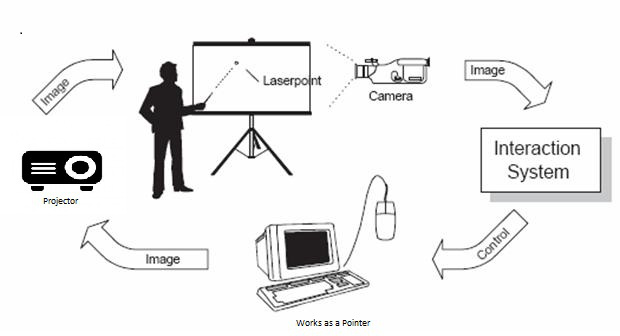
\includegraphics[width=0.48\textwidth]{abc.jpg}
	\caption{Laser Pointer based Interactive Projector System}
\end{wrapfigure}

Interactive Projectors makes sense for the users who want the combination of projector and interactive whiteboard in an individual system. Such interactive projectors are scoped under \textbf{Human Computer Interaction(HCI)}, especially vision-based HCIs. \textbf{Computer Vision(CV)} is an integral part of the interaction. It acts as an apt mediator between the user interface and the computer, and sends the actions from the user into machine understandable format. Since here, there is not only the involvement of images and enhancements, or analysing them but would be emulating human vision(examples: object recognition, tracking,etc.).

In the context of Nepal, in rural classrooms, such audio-visual learning tool would be a boon to students where they no access to the know-hows of the outside world easily. Additionally, this would be a cheaper solution compared to the installments of numerous computers in a school. 


\newpage
\section{Literature Review}
The current prototype can run off a rechargeable 12V battery, has the capability to access the World Wide Web, has readily available offline content, via established partnerships, and has an extremely easy to use interface. The device is contained in a single unit with replaceable external components (i.e. keyboard, remotes), consumes less than 100 W of power, and will cost only USD 300. The system is about the size of a shoebox. 
As seen in the Figure 2, the existing Looma system functional parts can be listed as:
\subsection{Looma and Wand Details}
\begin{itemize}
\item300 lumens projector
\item Internet Connected 
\item Wireless Wand control from front of room
\item Audio output for large room setting
\item Rechargeable 12V battery (8Hrs per charge)
\item Computer: Pandaboard
\item External ports: 1 Ethernet
\item Custom power supply (12V in 5V, 12V, 19.5V out)
\item Hacked Wii IR Camera and Wii wands
\end{itemize}
\begin{figure}[htp]
\centering
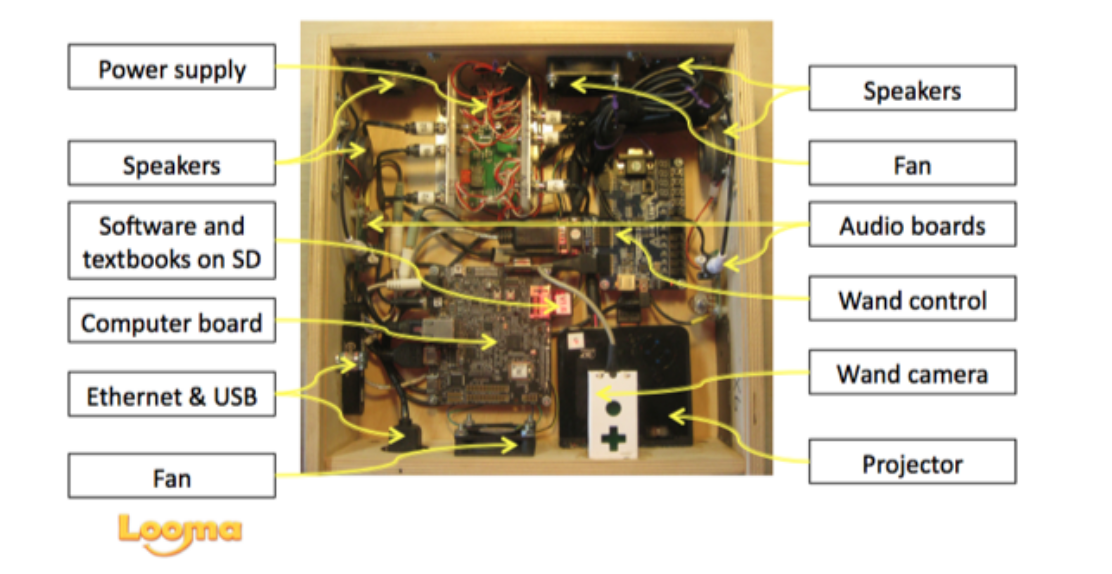
\includegraphics[scale=0.22]{looma.png}
\caption{Hardware and Electrical parts of Looma system}
\label{}
\end{figure}
\newpage
Wand control descriptions:

\begin{itemize}
\item Wand shown in the figure is a 3D printed IR light source
\item The wand design uses 555 timer to turn the IR light source on/off at a pre-determined frequency such that the blink can be interpreted as a click on the device
\item Current design uses Nintendo Wii IR camera, which are scavenged from Wii motes
\end{itemize}
\begin{figure}[htp]
\centering
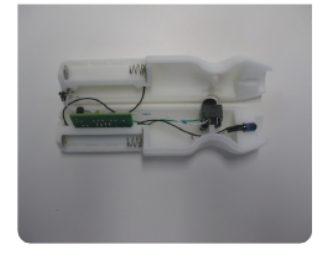
\includegraphics[scale=0.4]{wand1.png}
\caption{3D printed hacked Wii Remote wand}
\label{}
\end{figure}

\newpage
\subsection{System Operation Description}
The existing system uses Wii Remote to interact in the audio-visual device. This system uses an Wii IR camera which picks up the infrared light source, and tracks it using its MOT (Multi-Object Tracking) processor present in the camera chip as shown in the Figure 4. Wii IR Camera gives out a pre-set I2C address so the interface board needs an I2C multiplexer. To convert the I2C output to serial, and to demultiplex the signals, the system has been using an FPGA board. 

\begin{figure}[htp]
\centering
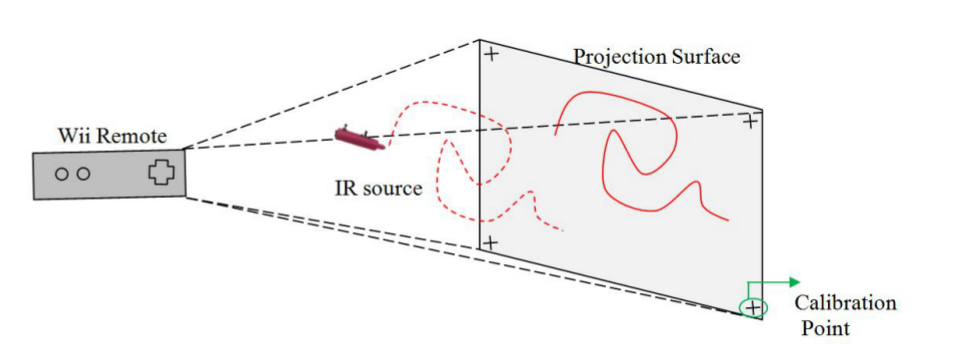
\includegraphics[scale=0.35]{wiiiii.png}
\caption{Illustration of how the movement of infrared is picked up by the Wiimote}
\label{}
\end{figure}
\subsection{Problem Statement}
 However, some of the system issues which can not be ignored are:
\begin{itemize}
\item \textbf {Drawing in the Whiteboard:} While drawing in the LOOMA software, the tracking of the IR led is very unreliable and the drawings are not made as expected.
\item \textbf{Use of Pre-built MOT processor:} There is the use of inbuilt MOT processor in the camera chip, which does part of the image processing and tracking and sending coordinates. In the case of errors, its response can not be modified to remove errors which makes it inefficient
\item \textbf{Errors not detectable:} Since the Wiimote used IR to move the mouse, the location of the IR on the screen is not visible with the naked eye thus making errors not detectable 
\item \textbf{Unavailability in the market:} Wiimote IR camera chip being used in the system can not be readily bought in the open market which makes it difficult to mass produce the system
\item \textbf{Coverage and Difficult to Interact:} Wii wand is not interactive enough and works effectively only within the projected screen space which makes interacting with the screen difficult and not intuitive

\end{itemize}

In short, hacked Wii Remotes along with the FPGA board has been adding up to the cost significantly. In addition, the system is not very stable and is inefficient to use as points aforementioned, thereby leading to the research on alternative vision-based HCIs and our project is an effort to get a prototype of one such alternative.

\newpage
\section{System Block Diagram}
\begin{figure}[htp]
\centering
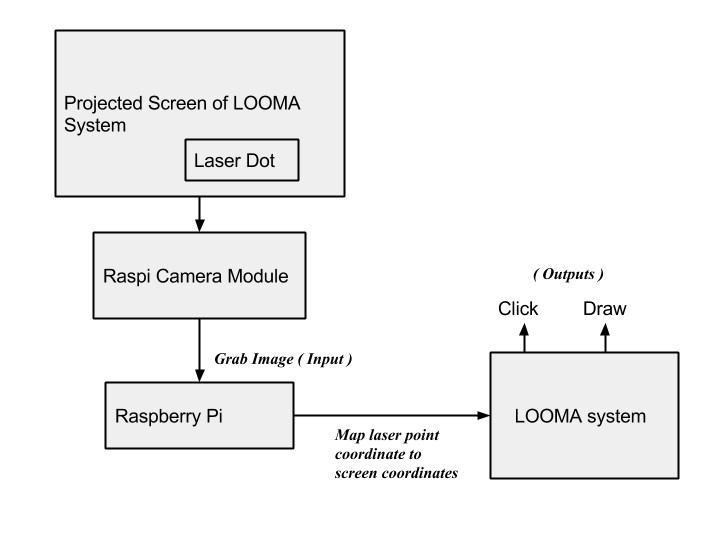
\includegraphics[scale=0.45]{block_diagram.png}
\caption{Block Diagram of the working of the LP-HCI-CV}
\label{ }
\end{figure}
\subsection{System Block Explanation}
\subsubsection{Projected Screen of Looma}

The Looma software runs on Looma hardware or Ubuntu. The display resolution of the screen is given by X = 1280 and Y = 768, and the display width is 60. Once the device is up, there are options of whether to use the wand or not use the wand. In the projected screen of Looma, ther is a custom made user interface for the teaching materials for the students as seen in Figure 6 below.

\begin{figure}[htp]
	\centering
		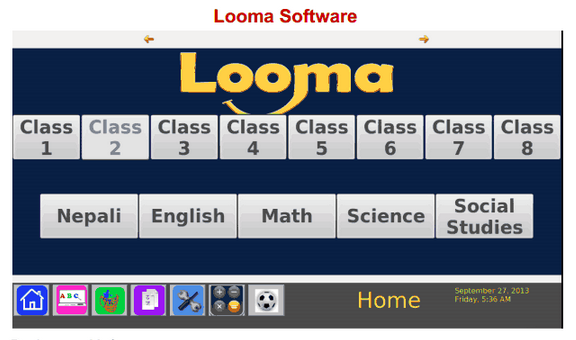
\includegraphics[scale=0.19]{loomasoftware.png}
	\caption{Looma Software}
\label{}
\end{figure}

\subsubsection{Raspi Camera Module}
Raspberry Pi Camera Board Module supports a full HD (High Definition) video streaming at fps of 30 with its 5 megapixel native resolution, and the sensor capable of 2592-1944 pixel static images. Raspberry Pi Camera Board Module was opted instead of normal USB web camera. 

The software of Raspberry Pi utilizes Rpi GPU (Graphical Processor Unit) when using Raspi Camera Module. So for example encoding \emph {h.264}, video has low impact on the CPU (Central Processor Unit) usage. Also, it has an excellent resolution of 5 Megapixels, which is higher than most USB webcams. It also has an excellent daytime image quality. If we use USB Webcam, it will have a very slow frame rate video and the CPU usage will be quite high. RPi does not have enough CPU horsepower to do higher frame rates, resolution and advanced video compression. 

\subsubsection{Using Picamera}
Raspberry Pi camera module will use \emph{Picamera 1.2} by Dave Hughes, recently released on February 06, 2014. This is a pure Python interace to the camera module. Having this interface is a boon since, up until now, the command line syntax needed to be utilized for taking still images and video taking and any changes to the camera's intrinsic features would have required a restart of the camera interfaces and Rpi.

\subsubsection{Raspberry Pi}
Raspberry Pi is a single-board computer with processor, memory, I/O ports and many more features, which together make it a functional computer for a wide range of applications in robotics. It is so simple than any logical person can program it, even it is for the first time when you work with a single-board computer.The ARM powered minicomputer is a platform with enormous possibilities and powerful enough to run many of the same programs as computer. Raspberry Pi serves as a wonderful platform for computer vision algorithms given its size, wonderful camera board and portability. Using the Picamera module, we took raw byte streams of the projected screen, and converted them to OpenCV (Open Computer Vision) object before doing further image processing algorithms.

\subsection{System Design and Description}
As seen in the Figure 5 and Figure 7, the camera will be taking in the images of Looma continually and the raspberry pi will be applying the laser detection and click action detection algorithm on the images. The image processing part will be done in the raspberry pi. Initially, the projected screen must be intially checked for any distortion and warpness. Depending on the distortion, linear and non-linear screen coordinates mapping matrix will be used. If no such distortion is present, simple linear transformation matrix will be able to map the coordinates to move the mouse pointer accordingly. However, for distortion filled projected screen, non-linear mapping transformation need to analysed and assessed. Once the mapping matrix has been understood, the raspberry pi takes in the images and works on the projected screen extracted as the region of interest. Now, all the image processing algorithms will be analysed within this ROI (Region of Interest).

\begin{figure}[htp]
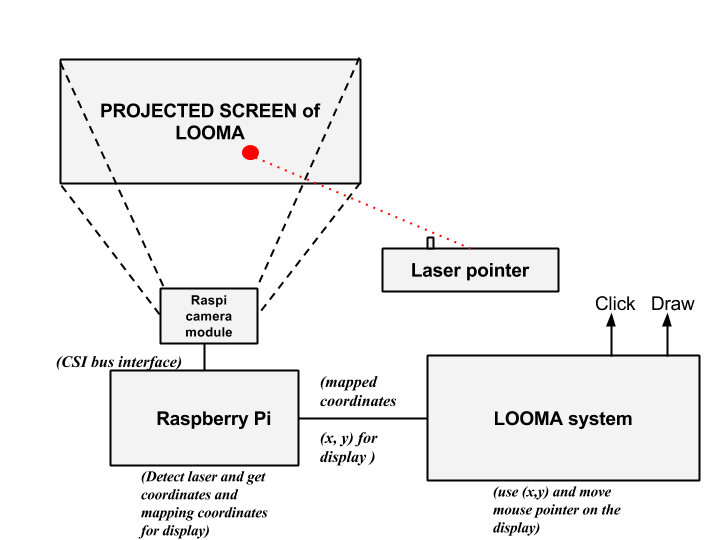
\includegraphics[scale=0.5]{proposed_system}
\caption{Overall System}
\label{Proposed Block Diagram}
\end{figure}

Next task is to understand the actions of the laser pointer and obtain the coordinates of it and feed it to the Looma System. The actions of the laser pointer are either simple pointing or clicking. Simple pointing will be based on the tracking of the laser pointer in the projected screen and updating the mouse pointer. Clicking of the laser pointer will be understood by the software when the laser pointer is turned on and off for a certain number of times. This on and off pattern of the laser pointer is checked in a number of frames on the same location in the image. This will be implemented as a software click and the mouse click action is done in the Looma software. 


In the Looma System, we will have the system taking in our actions and coordinates and updating its mouse pointer to do the desired mouse actions. Raspberry Pi will be connected to the Looma system through the USB to Serial Port converter wire, with the USB being the part of Raspberry Pi and the Serial Port being the part of the Looma System.

\newpage
\section{Project Completed in the Seventh Semester}
\subsection{Summary of Work Completed}
During the work on the Major Project Part A, our team was successful in detecting laser pointer motions and moving mouse accordingly. In addition, for detection of laser pointer in all sorts of lighting conditions, we have programmatically changed the camera exposure settings to get laser pointer detected properly. After each milestones achieved, we have reported to the Looma representatives of our progress as well. We have enlisted the following project milestones, which will provide an overview of how our work was carried out in different stages and the overall work breakdown process:
\begin{enumerate}

\item Intially once we obtained the Looma hardware, the hardware was tested for any defects. Of the two wands, one of them did not work. We were able to run Looma software successfully using the wand over a period of \emph { 2 }days of learning. 

\item The most important part of our project was detection of laser pointer. We were able to detect laser pointer by cascading a number of image processing algorithms of which the HSV color segmentation played a pivotal role. Since we were using red colored laser pointer, we needed to analyse the HSV (Hue Saturation Value) color value of red colored laser pixel. Once we were able to identify the range of red color for our laser pointer, we were able to obtain the laser pointer coordinates in a span of \emph {1 and half week}. 

\item The second most important part was that laser pointer be detected in all sorts of lighting conditions, no matter if the room is full lit or dark. The camera must be able to detect the laser pointer at all conditions. For that we have been able to dynamically change the camera exposure depending on the light conditions. We completed this in a span of 2 weeks including the research and porting of codes from computer to Raspberry Pi. Also, we needed to wait for hardware deliveries which prolonged testing on Raspberry Pi for longer than \emph {2 weeks}.  

\item We needed to signify clicks using the laser pointer and for that we were able to customize a circuit that switches off led for a specific number of time using a 555 timer in astable mode. Varying the resistors and capacitors on the circuit required quite a bit of tuning and this task was achieved in a span of \emph {a week}. 

\item Lastly we were able to move the mouse pointer in accordance to the laser pointer coordinates in the image space onto the display space using a simple linear transformation matrix. We were able to do this within a span of \emph { 2 days}.

\end {enumerate}
\subsection{Preliminary Experimental Work}
\subsubsection{Extraction of Region of Interest}

The projected screen is our region of interest, ROI, from the whole of the image captured by the camera. The region of interest extracted is also called \emph{segmentation}, and the features of these ROI's are used as input data for further calculations. So first, we tried to identify the projected screen from the wall. For that, thresholding was done, where a threshold value is used to turn a graylevel scale image to binary image. We binary thresholded the image based on the brightness contrast of the projected screen with the wall. From the obtained processed image, all the contours were found out. From all these contours, the contour with the largest area was taken and a bounding rectangle was approximated on it to obtain the rectangular coordinates of the projected screen. This gave us the region of interest from the over all image capture. Despite this being our ROI, it will need to be checked for distortion, and necessary transformation needs to be applied to map the coordinates accordingly. Other than that, the images can be assumed to be taken by camera as planar, and not distorted. The extracted ROI of the projected screen can be viewed in Figure 8.

\begin{figure}[htp]
\centering
\includegraphics[scale=0.17]{bounding.jpg}
\caption{Extraction of ROI}
\label{}
\end{figure}

\subsubsection{Movement of Mouse Pointer}
To move the mouse pointer as per the laser pointer movements, we used the Python X library. It is a fully functional X client library intended for Python programs working as client programs to communicate with the X server via the X protocol. It runs on Linux using XFree86 as the server and most Unices.

The X Window System is a network--transparent window system that was designed at MIT. X display servers run on computers with either monochrome or color bitmap display hardware. Once the connection has been set up, we can use the Xlib macros and use functions to get the information about the current display. Similarly, using the X objects, we moved the mouse pointer as by sending coordinates to the appropriate functions, a mouse poiner moving code of which has been shown in Appendix A1.

\subsubsection{Using Raspberry Pi}
\begin{enumerate}
\item \textbf{Connecting Raspberry Pi to other OS to program in linux:}
VNC\textbf {(Virtual Network Computing)}
allows to see Pi’s desktop and control it remotely using another computer running Mac OS X, Windows or Linux. The VNC server software runs on  RPi, accesses it by running VNC client software on other devices as shown in Figure 9.

\textbf{VNC Server:}
Using the TightVNC server software the following commands are run from the command line:
\begin{itemize}


\item \textbf{Installallation of tight VNC:} \emph{sudo apt-get install tightvncserver} and the program is run: \emph{tightvncserver}.A VNC session is started: \emph{vncserver:1 --geometry 1024*728 --depth 24}

\end{itemize}
\textbf{NOTES:}
The session’s resolution is configured after the geometry argument.1024*768 is used above.The Rpi is capable of full HD 1920*1080.
Colour depth is specified by the --depth argument. 24-bit colour depth is used above. 16-bit cn be used instead to reduce network traffic.
More than one VNC sessions can be started by running subsequent vncserver commands, by incrementing the first digit: e.g. \emph{vncserver :2} for a second, \emph{ vncserver :3} for a third.

\textbf{VNC Viewer/Client:}
A lot of VNC clients can be used. We used TightVNC. It has a free client application, there’s a native Windows version and a Java version, which run on any desktop/laptop system.
To connect to RPi:
\begin{enumerate}
\item RPi's IP address is obtained by command "ip addr show" in command prompt.
\item Our client is connected to the IP address obtained from 1.
\item Then IP address followed by \emph{:x}, for example \emph{192.168.1.150:1} where "x" is the session no. is entered.
\item It will prompt  to create a password. Passwords can be at most 8 characters long.
\item Once we have entered a password the VNC server is now running in the background of your Raspberry Pi's operating system. Now we can use any computer on  network with a VNC client to remotely access the Raspberry Pi as shown in Figure 9.
\end{enumerate}

\end{enumerate}
\begin{figure}[htp]
	\centering
	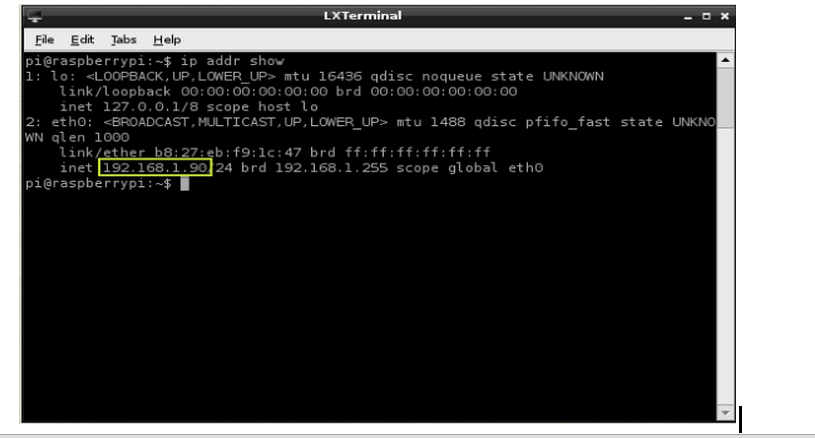
\includegraphics[scale=0.3]{rpi.png}
	\caption{VNC settings}
	\label{}
\end{figure}

\subsubsection{Detection of Laser Pointer:}
\begin{enumerate}
	\item \textbf{HSV segmentation:}

	In the process to detect the laser pointer we used the HSV segmentation and performed histogram analysis and obtained results as shown in Figures 11 and 12 below.
	The basic steps followed were:
	\begin{itemize}
	\item Capture the frame at each instant of time.
	\item As the captured image in opencv is in RGB (Red Green Blue) form as default , we convert it into HSV value.
	\item From the HSV value we made the value of the red color of the pointer as the default such that it can be used for further operations.
	\end{itemize}
	\emph {Why is HSV used instead of RGB value?}
	HSV separates the color component and the image intensity because of which we can operate on each image intensity as per our requirement without changing the color information which plays a vital role in color detection. RGB is the way computers treats color, and HSV try to capture the components of the way humans perceive color.   
	\item \textbf{Masking the image:}
		We obtained the threshold of the laser pointer’s color. Using the threshold range, the mask was created. The image and the masked image were operated with bitwise AND operation. Now, only the laser pointer remains in the image, remaining section is masked as black.

	\item \textbf{Canny Edge detection:}
For the edge detection we used canny edge detection algorithm.It is a multi-stage algorithm and we will go through the following stages:
\begin{enumerate}
\item \textbf {Noise Reduction}
Since edge detection is susceptible to noise in the image, first step is to remove the noise in the image with a 5x5 Gaussian filter.
\item \textbf{Finding Intensity Gradient of the Image}
Smoothened image is then filtered with a Sobel kernel in both horizontal and vertical direction to get first derivative in horizontal direction (Gx) and vertical direction (Gy). From these two images, we can find edge gradient and direction for each pixel as follows:
\begin{figure}[htp]
\centering
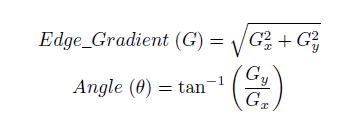
\includegraphics[scale=0.7]{canny.png}
\caption{Intensity Gradient and Direction}
\label{}
\end{figure}

Gradient direction is always perpendicular to edges. It is rounded to one of four angles   representing vertical, horizontal and two diagonal directions.
\item \textbf{Non-maximum Suppression}
After getting gradient magnitude and direction, a full scan of image is done to remove any unwanted pixels which may not constitute the edge. For this, at every pixel, pixel is checked ­if it is a local maximum in its neighborhood in the direction of gradient.

\item \textbf{Hysteresis Thresholding}
This stage decides which are all edges are really edges and which are not. For this, we need two threshold values, minVal and maxVal. Any edges with intensity gradient more than maxVal are sure to be edges and those below minVal are sure to be non-edges, so discarded. Those who lie between these two thresholds are classified edges or non-edges based on their connectivity. If they are connected to “sure-edge” pixels, they are considered to be part of edges. Otherwise, they are also discarded.
\end{enumerate}

	\item \textbf{Contours:}
		We found the contours of the image output from the step 4. Hence, laser spot was found and a contour and laser center was drawn out as shown in the diagram below:
\end{enumerate}

\begin{figure}[htp]
	\centering
	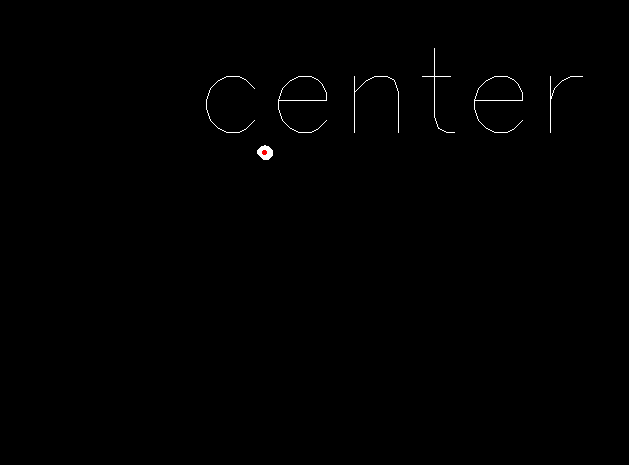
\includegraphics[scale = 0.6]{center.png}
	\caption{Laser pointer center}
	\label{}
\end{figure}

\begin{figure}[htp]
	\centering
	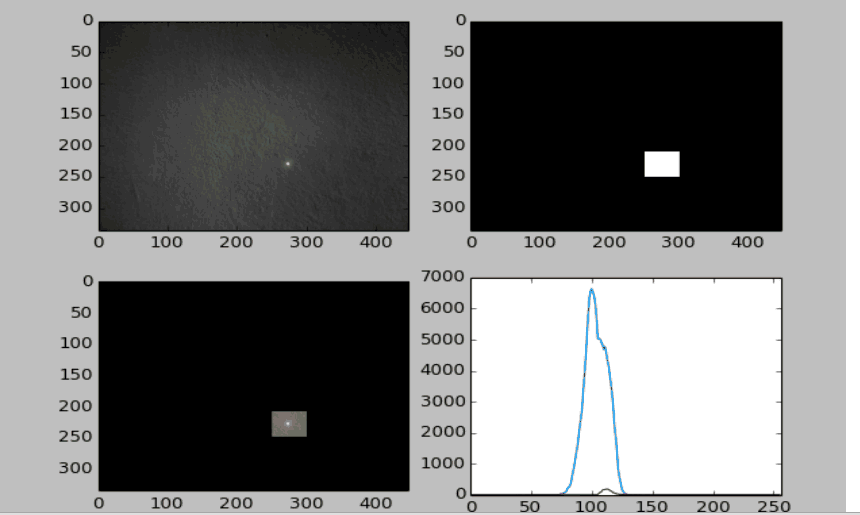
\includegraphics[scale=0.35]{histogram.png}
	\caption{Histogram Analysis of Laser Pointer}
	\label{}
\end{figure}


\newpage
\subsection{Works Accomplished}
\subsubsection{Detection of Laser Pointer and Mouse Movements}
	Integrating the above two codes of laser pointer detection and mouse handler into one, we were able to move the mouse pointer as per the laser pointer coordinates. Assuming that the camera captures the image from the wall without distortion, a simple linear transformation was carried out, where the laser pointer position in the image taken was mapped to the display resolution of our computer. The supporting code can be followed in Appendix A2.

	As we can understand from the code, from the camera's capture properties, we have extracted the width and height of the image being captured. A simple scalex and scaley have been derived with 1366 and 766 being the display resolution of our sample display device. Once the laser pointer coordinates are found, the transformation is carried out and the mouse pointer coordinates is updated simultaneously so as the laser pointer moves, the mouse pointer coordinates gets updated and it moves with the laser motion. The mapping code can be followed in Appendix A3.

\subsubsection{Dynamic Exposure Correction}
	Correct exposure configuration of the camera can improve the color detection of laser spot. In Raspberry Pi, dynamic exposure correction was done as per need by modifying its camera capture property, which is its camera exposure compensation parameter. Here, the projected screen was captured, and the camera exposure value were modified until color of laser spot was the brighest color in the inpurt image. On every frame captured, the average of the value channel of the image was compared with the preset threshold for seeing laser spot. If the average of the value channel was greater than this threshold,the camera exposure level was decreased accordingly. A sample exposure correction code can be viewed on Appendix A4.

\subsubsection{Porting of Code to Raspberry Pi}
	All the codes run and tested in our computer using inbuilt webcam was ported to Raspberry Pi and run using picamera module for using the Raspberry Pi Camera Board Module. A sample picamera module code for converting to OpenCV object has been shown in Appendix A5.

\subsubsection{Design Calculations of 555 timer}

	A simple led circuit is used for the pointing purpose in the wand. To avoid leaving the wand on at all times, a circuit break can be introduced using a simple one-way switch. However, for the clicking purpose, the led circuit must be modified for the system to understand and implement the click. 
	One of the method to signify a click is to switch off the led for a short time but this leads to misintended clicks whenever the led is out of sight of the system. Thus, in order to avoid such errors, the led is made to blink for a specific number of times at a predetermined frequency which is understood by the system as a click. In order to implement this, a flashing led circuit was designed using a 555 timer. 
	The 555 timer is operated in astable mode and outputs rectangular pulses of certain frequency. The frequency is determined by the values of components kept in between the pins of the timer. See Fig 13 and 14.


	The values of R1, R2 and C are set to obtain the required positive time interval(T1), negative time interval(T2) and frequency(f). The calculations are made as follows:

	\noindent
	T1 (ms) = 0.693 * ( R1 + R2 ) * C \\
	T2 (ms)  = 0.693 * R2 * C \\
	Frequency (KHz)  = 1.44 /( ( R1 + R2 + R2 ) * C)

\begin{figure}[htp]
	\centering
	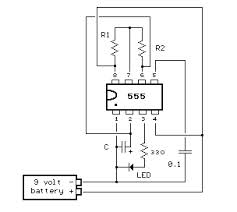
\includegraphics[scale=1]{blinking.jpg}
	\caption{555 Timer Calculation}
	\label{}
\end{figure}

\begin{figure}[htp]
	\centering
	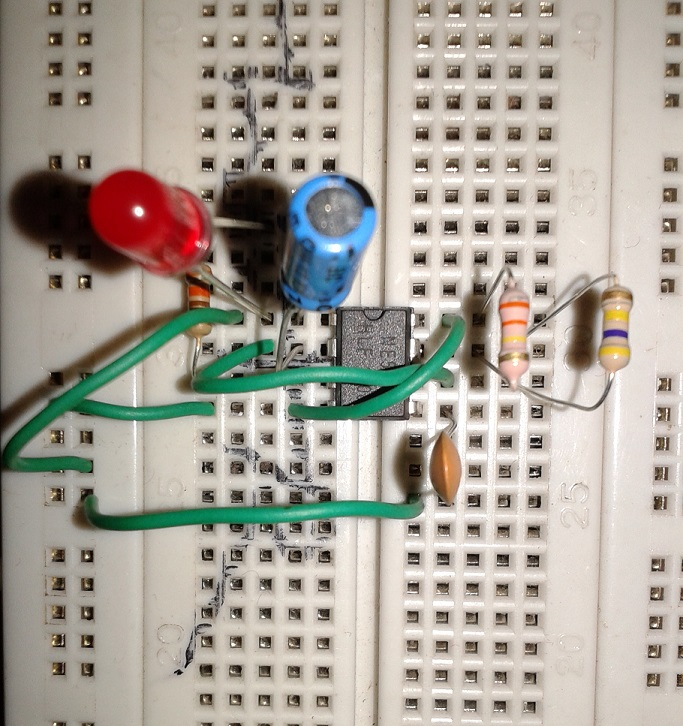
\includegraphics[scale=0.4]{circuit.jpg}
	\caption{Circuit Test on breadboard}
	\label{}
\end{figure}

	The values of the resistors and capacitor were varied until the required frequency and blinking intervals were obtained.
	By observation, we found out that R1 should be greater than 1K and C must be greater than 0.0005 uf for a proper working circuit.


\newpage
\section{Project Plans for the Eighth Semester}
	As per the second part of the project we have planned to work on integrating a robust laser pointer detection with mouse cursor movement in the Looma system itself. 

\subsection{Works to be done}

\subsubsection{Initial Calibration of Projected Screen}
	The image projected on the screen is not equal to the size of the computer image, but all the operations and analysis are to be performed with respect to the computer display(or camera frame). So for the calibration of the projector image, we need to map the point in the projector slide to pixel on the camera frame such that all the operations are done on the camera frame. For this mapping purpose, single projective transform will be used as the matrix. Our main calibration will be done on the basis of the linear mapping which works on the undistorted straight projection screen. 
	Although we will be using the linear mapping techniques, non-linear mapping techniques can also be used for the curved or uneven surfaces like curtains, as our projection screen may not always be a straight surface like wall.

\subsubsection{Finalization of Laser Detection Algorithm}
	Upto now, the laser pointer has been detected using HSV color based segmentation. However, the projected screen may comprise of many brighter pixels and red regions. Since the laser pointer center is perceived as white by the camera, they appear as complete white in bright white background. This led to the exposure correction of the camera. So color based segmentation can not be used as our primary technique of laser pointer detection. Currently, we have been able to change the camera exposure settings based on the intensity of light in the image taken. We are currently modifying the algorithm where first we are planning to check for bright pixels in the image and then only do color based segmentation of laser pointer.


\subsubsection{Communication between Looma system and RPi}
	Currently, the Looma software is obtaining the mouse coordinates through its serial port from the FPGA board using a serial to USB converter with serial end at the FPGA. Since the FPGA is now being replaced by the Raspberry Pi, the serial end will now be at the Pandaboard. Once the laser spot has been identified and the coordinates are obtained, they are sent from Raspberry Pi to the serial port of the pandaboard in the Looma system.

	In short, previously, FPGA (Serial Port) to Pandaboard (ttyUSB) whereas now, Raspberry Pi (ttyUSB) to Pandaboard (Serial Port). Using the coordinates received in the serial port, the Xlib of the Looma system is updated and desired mouse movements and actions are carried out.

\subsubsection{Documentation}
	All the researches and case studies conducted will be documented using standard Latex documenting software.

\newpage
\section{Project Timeline}
\subsection{Works Completed Timeline}
\begin{figure}[htp]
\centering
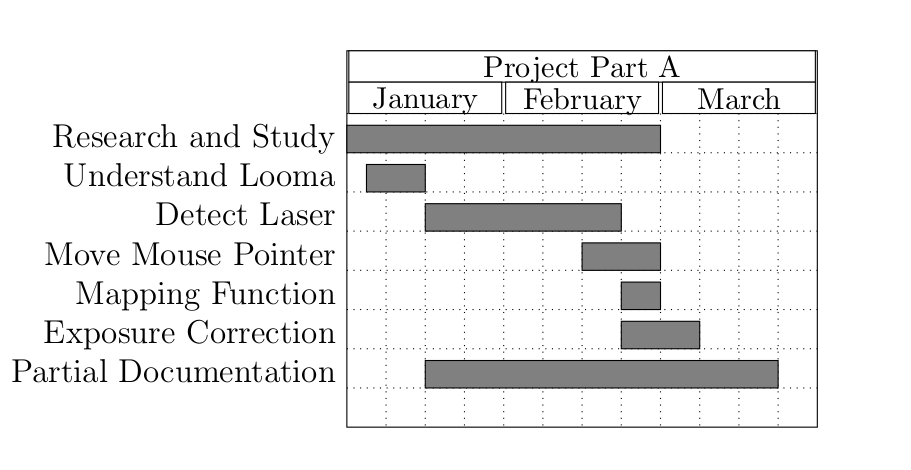
\includegraphics[scale=0.35]{reformed1.png}
\caption{Works Completed Timeline}
\label{}
\end{figure}
\subsection{Works Remaining Timeline}
\begin{figure}[htp]
\centering
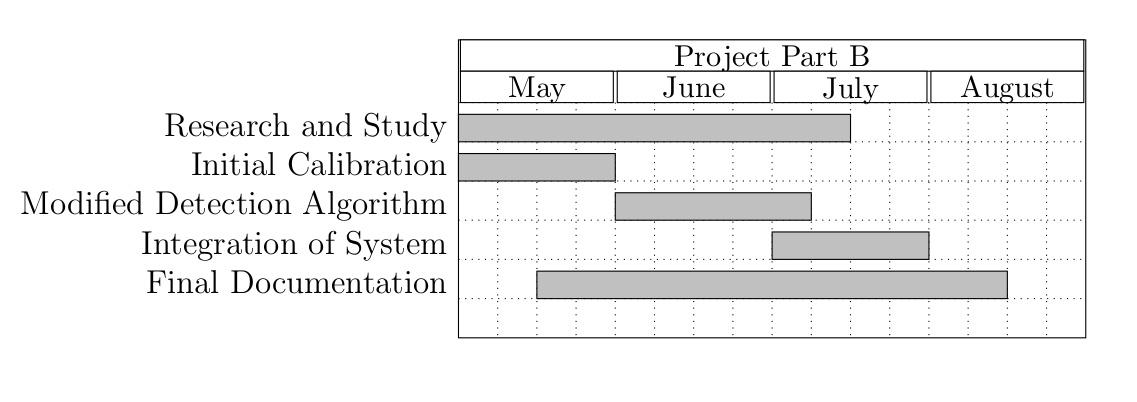
\includegraphics[scale=0.35]{final.png}
\caption{Works Remaining Timeline}
\label{}
\end{figure}
\newpage
\section{Bibliography}
\begin{enumerate}
\item Information and Communication in Technology (ICT) in Education Master Plan 2013-2017 
\item Kirstein and Muller, Interaction with a Projection Screen Using a Camera-Tracked Laser Pointer,University of Dortmund, Germany
\item Mikawa, M., Morimoto, Y., Tanaka, K.: Guidance method using laser pointer and gestures for librarian robot, IEEE-RO-MAN, September, 2010
\item Johnny Chung Lee, Hacking the Nintendo Wii Remote, Carnegie Mellon University, IEEE-CS,2008 
\item Kent L. Norman, Kirk D. Norman, University of Maryland, Comparison of Relative Versus Absolute Pointing Device2, May, 2010
\item Matej MESKO, Stefan TOTH, Laser Spot Detection, University of Zilina, Faculty of Management Science and Informatics (2013) 
\item Nicole M. Artner, Upper Austria University of Applied Sciences, Austria, A Comparison of Mean Shift Tracking Methods,(2011)
\end{enumerate}

\section{References}
\begin{itemize}
	\item \url{www.python.org}
	\item \url{www.raspberrypi.org}
	\item \url{www.simplecv.org}
	\item \url{www.villagetechsolutions.org/}
	\item \url{www.docs.opencv.org/}
\end{itemize}

\newpage
\section{Appendices}

\noindent
	
	\chapter{Appendix A1: Mouse Movements}
	\lstinputlisting[language=Python]
	{Xlib.py}
	\vspace{6mm}
	
	\chapter{Appendix A2: Laser Detection}
	\lstinputlisting[language=Python]
	{laser.py}
	\vspace{6mm}

	\chapter{Appendix A3: Scaling}
	\lstinputlisting[language=Python]
	{scale.py}
	\vspace{6mm}

	\chapter{Appendix A4: Exposure Correction}
	\lstinputlisting[language=Python]
	{exposure.py}
	\vspace{6mm}

	\chapter{Appendix A5: Using Picamera }
	\lstinputlisting[language=Python]
	{picamera.py} 

\end{document}
